
\chapter{Installing SCHC rules in openSCHC}\label{chap-rules}

SCHC is a protocol taking place between two SCHC entities connected via a link. Usually, one SCHC entity is implemented in a constrained end-device and the other one is implemented in a core equipment acting as a router. To allow the pair to perform the same action, or more precisely an action on one end and the inverse action and the other end, e.g., compression and decompression, or fragmentation and reassembly, a common set of rules must be shared between these two entities.

~

The distinction between a device and a core tells which communication is uplink (from the device to the core) and which is downlink (opposite direction). The device usually contains a small set of compression of fragmentation rules tailored to the traffic generated and received by that device only. Conversely, the core instance of SCHC must know all the devices' rule sets. Even if all the devices happen to be identical, the SCHC core treats each device as if it were unique. 

\section{Rule ID's}

Rules are identified by a \Index{rule ID}. A rule ID is a binary sequence that must be unique within the scope of the link between a device SCHC instance and a core SCHC instance. \rfc{8724} does not specify the length of the rule ID's: the lengths are chosen as the rules are defined, the lengths can even be different for different rules within the same set. Within a set of rules, the rule ID representations must not overlap, when read from left to right. 
For instance:

\begin{itemize}
\item\texttt{0} and \texttt{111111} are two valid rule ID's
\item \texttt{01} and \texttt{0101} is not a valid pair of rule ID's within the same set: on receiving the sequence of bits 0101 (from left to right), it is impossible to tell which rule is being received.
\end{itemize}

~


Rule ID's could be described using their binary representation but, for compactness, the decimal notation \texttt{rule ID value/rule ID length} will be used in this book . For instance, \texttt{3/8} indicates a rule ID represented on 8 bits and having a decimal value of 3 (right-aligned), which is equivalent to the \texttt{00000011} binary representation.

~

Pay attention that this notation can be misleading: for example, \texttt{1/2} and \texttt{5/4} don't look like they overlap, even though they do (binary \texttt{01} and \texttt{0101}); as another example, the pair \texttt{12/4} and \texttt{12/6} looks suspicious even though it is perfectly valid (binary \texttt{1100} and \texttt{001100}).

\begin{figure}[tbp]
\centerline{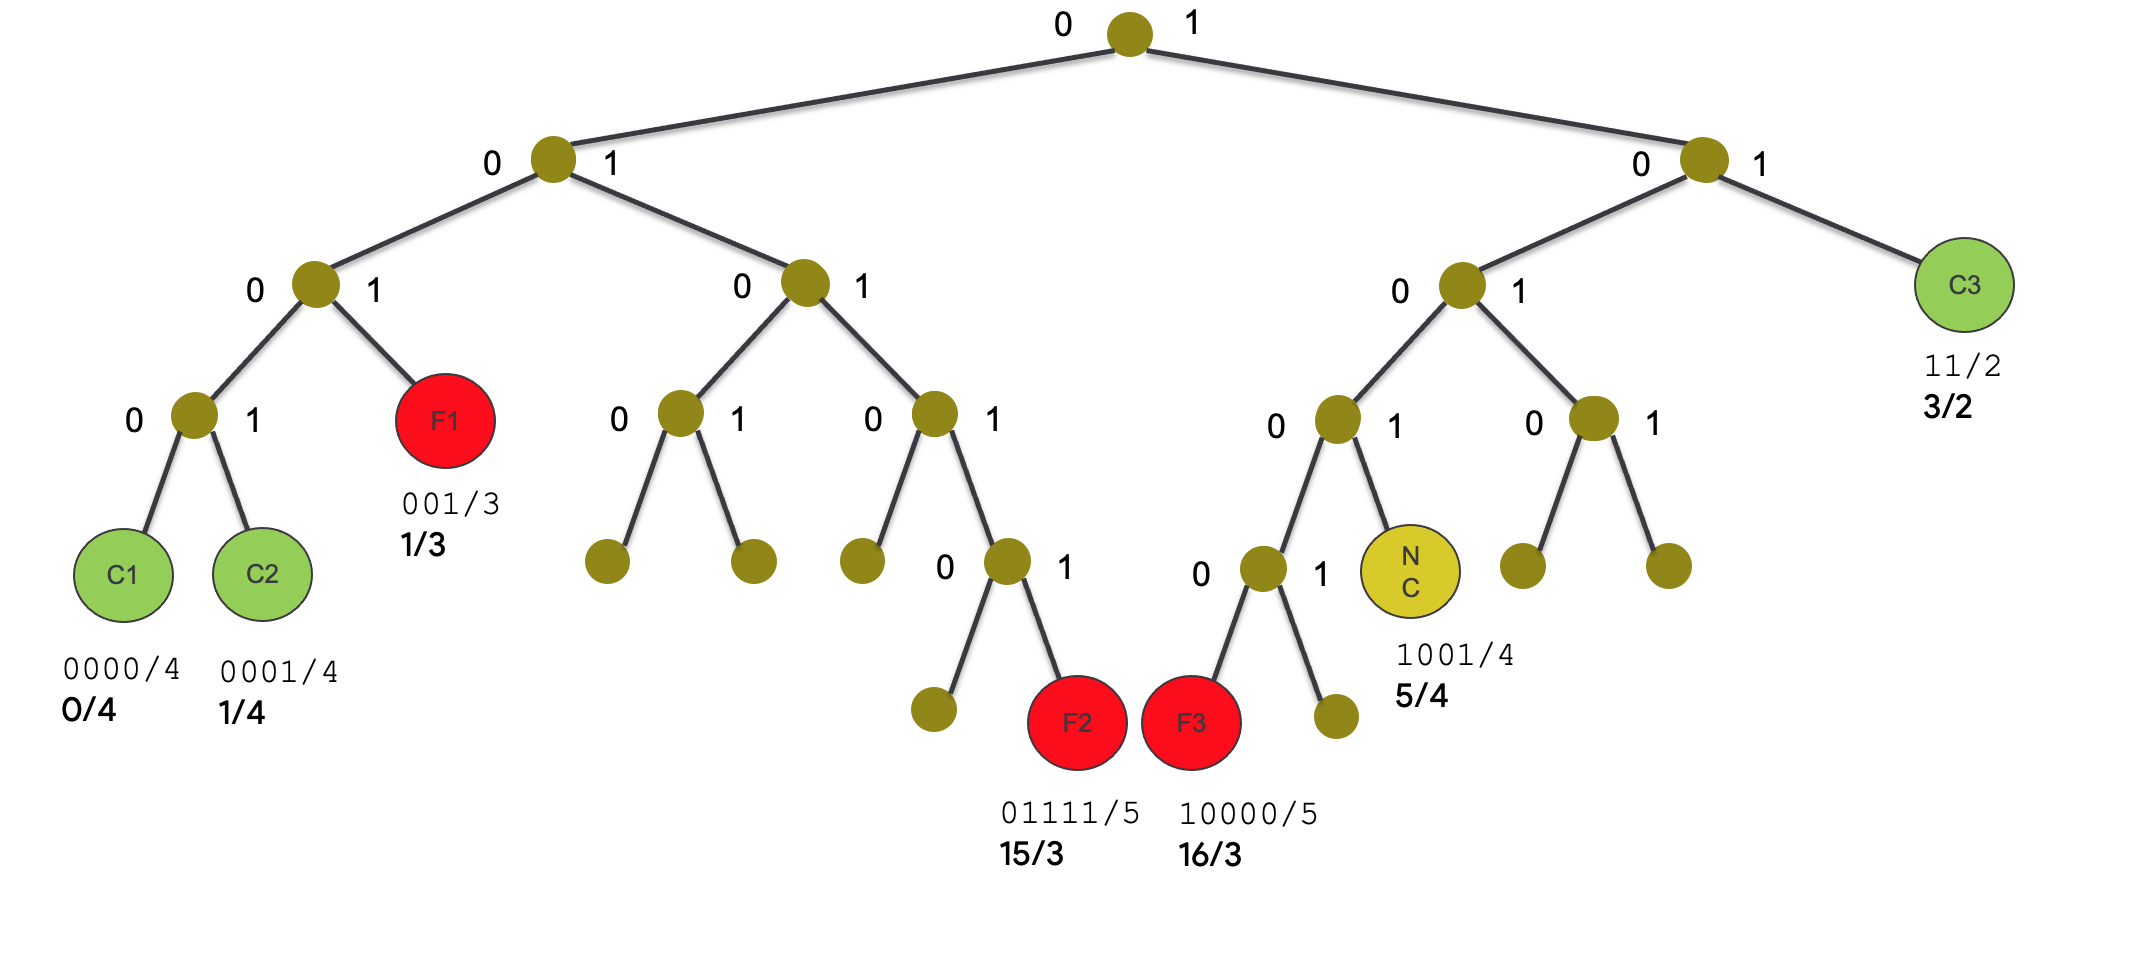
\includegraphics[width=1\columnwidth]{Pictures/binary-rule.png}}
\lge{\caption{Example of binary tree associated to rule IDs}}
\label{fig-base64}
\end{figure}

\section{Rules structure}\label{OpenSCHCRules}

In the openSCHC implementation of SCHC, a rule is described with a JSON object, and the rule ID is expressed with the decimal notation introduced above:

\begin{lstlisting}[backgroundcolor=\color{yellow}]
    {
    "RuleID" : 12,
    "RuleIDLength" : 4
    }
\end{lstlisting}

There are three different rule formats. The first one is used for \Index{Compression} Rules, which contain the \texttt{Compression} keyword followed by an array, as shown in the minimal example below: 

\begin{lstlisting}[backgroundcolor=\color{yellow}]
   {
   "RuleID" : 12,
   "RuleIDLength" : 4,
   "Compression" : []
   }
   
\end{lstlisting}

The second format is used for \Index{Fragmentation} rules, which contain the \texttt{Fragmentation} keyword followed by an object describing the fragmentation parameters:

\begin{lstlisting}[backgroundcolor=\color{yellow}]
    {
    "RuleID" : 12,
    "RuleIDLength" : 6,
    "Fragmentation" : {
      "FRMode" : "NoAck",
      "FRDirection" : "UP"
    }
\end{lstlisting}

Finally, the \Index{\texttt{NoCompression}} keyword is used to describe the mandatory default rule that SCHC resorts to for sending a packet when no valid compression rule was found to compress it.


\begin{lstlisting}[backgroundcolor=\color{yellow}]
   {
   "RuleID" : 666,
   "RuleIDLength" : 10,
   "NoCompression" : []
   }
\end{lstlisting}

The fragmentation, compression and no-compression rules share the same rule ID space: the same rule ID cannot be used for both a compression rule and a fragmentation rule, for example. 

An observant reader may have noticed that the fragmentation rule description includes a direction indicator. 
Indeed, SCHC compression rules are bi-directional (the same rule can be used to compress a packet flowing from a device to the core or from the core to the device), but fragmentation rules are oriented (they only apply to either uplink of downlink traffic).  

~



\section{The Rule Manager}

The \Index{Rule Manager} plays an important role in the openSCHC implementation of SCHC. It has multiple goals:
\begin{itemize}
    \item check for the correctness of the rules external description,
    \item add default parameter values, which allows simplifying the rules external description,
    \item import external rule descriptions into internal storage,
    \item display the rules in the  store in a more compact format than JSON,
    \item find in the store a valid rule to compress or fragment an incoming packet with,\footnote{TODO: find a good rule, or better yet, the best rule, instead of the first valid one in the store.}
    \item retrieve a rule from the store by its rule ID.
\end{itemize}

\subsection{Adding Rules into the Rule Manager}\label{RuleDefinition}

Listing \ref{rm1.py} shows a simple python program used to manage the two rules described in \ref{OpenSCHCRules}. 

\pythonlst{rm1.py}

It first imports the \texttt{gen\_rulemanager} module, which defines the \texttt{\pfunction{gen\_rulemanager}{RuleManager}} class. 

~~


The \texttt{\pfunction{gen\_rulemanager}{Add}} method adds a new rule into the store.

~~~

The \pfunction{gen\_rulemanager}{Print} method displays the following:

\begin{termc}[backgroundcolor=\color{palerod}, basicstyle=\ttfamily\tiny, escapechar=@]
****************************************
Device: None
/-------------------------\
|Rule 12/4          1100  |
|---------------+---+--+--+------------------------------+-------------+----------------\
\---------------+---+--+--+------------------------------+-------------+----------------/
/-------------------------\
|Rule 12/6        001100  |
!=========================+=============================================================\
!^ Fragmentation mode : noAck    header dtag 2 Window  0 FCN  3                     UP ^!
!^ No Tile size specified                                                              ^!
!^ RCS Algorithm: crc32                                                                ^!
\=======================================================================================/
\end{termc}

Compression rules normally contain header field descriptors (omitted in this simple example) and Fragmentation rules contain the fragmentation parameters. Note that, for the fragmentation rule used here, the Rule Manager added some default parameters corresponding to the \Index{no Ack} behavior of SCHC.



\subsection{Adding a Set of Rules}

A device should contain a set of rules related to compression and fragmentation. In openSCHC, the SoR (\Index{Set of Rules}) is a JSON array. The following program has the same behavior as the one shown in \ref{RuleDefinition}, but the rules are added with a single method call, using an array.

\pythonlst{rm2.py}

\subsection{Attributing a Set of Rules to a Device}

You may have noticed that, in the previous examples, the device was displayed as None. This is appropriate when SCHC is instantiated on a device, since there is no ambiguity as to which device the rule set applies to. Conversely, when the SCHC instance resides on the core network side, each set of rules must be associated with a distinct device.

In openSCHC, the \Index{DeviceID} is structured as a link technology and an identifier within that link technology: 
\begin{itemize}
\item if the link technology is a \Index{UDP tunnel} (as in the test platform described in Chapter~\vref{chap-plat}), the technology keyword is \texttt{udp} and the identifier is the device-side tunnel endpoint IP address, followed by the port number used on that endpoint. A full DeviceID would therefore be, for instance, \texttt{udp:83.199.24.39:8888}\footnote{If the device is behind a NAT, the IP address used must be the global address assigned to the NAT.}. 
\item for \Index{LoRaWAN} (\textit{not yet implemented}), the technology keyword is \texttt{lorawan} and the identifier is the \textit{devEUI}.

\end{itemize}

~~

While being stored into the rule manager via the the \pfunction{gen\_rulemanager}{Add} method, rules can be attributed to a DeviceID as follows:

\begin{termc}[backgroundcolor=\color{palerod}, basicstyle=\ttfamily\small, escapechar=@, language=Python]
RM.Add(device="udp:83.199.24.39:8888", dev_info=[rule1100, rule001100])
\end{termc}

Alternately, the following JSON structure could be used:

\begin{termc}[backgroundcolor=\color{yellow}, basicstyle=\ttfamily\small, escapechar=@]
{
    "DeviceID": "udp:83.199.24.39:8888",
    "SoR" : [ ..... ]
}
\end{termc}

\subsection{Importing rules from a JSON file}

Rules can also be described in a JSON file, in which case the Rule Manager\texttt{Add} method is used with the \texttt{file} argument. For instance:

\begin{termc}[backgroundcolor=\color{palerod}, basicstyle=\ttfamily\small, escapechar=@, language=Python]
rm.Add(file="icmp.json")
\end{termc}

\section{Conclusion}

We have reviewed how rules are structured and how they can be added to the rule manager store. Let's now try to compress and fragment some traffic.

